\documentclass[]{scrartcl}

\usepackage{latexki}
%\lecturer{}
\semester{Sommersemester 2008}
\scriptstate{incomplete}

% Use utf-8 encoding for foreign characters
\usepackage[utf8]{inputenc}

% Setup for fullpage use
\usepackage{fullpage}

% Mathematical symbols
\usepackage{amssymb}

\usepackage[usenames]{color} 

% Uncomment some of the following if you use the features
%
% Running Headers and footers
%\usepackage{fancyhdr}

% Multipart figures
\usepackage{subfigure}

% More symbols
\usepackage{amsmath}
\usepackage{amssymb}
\usepackage{amsthm}
%\usepackage{latexsym}

% We want publication-ready tables.
\usepackage{booktabs}
\usepackage{multirow}

% Surround parts of graphics with box
\usepackage{boxedminipage}

% Package for including code in the document
\usepackage{listings}

\usepackage{hyperref}

% If you want to generate a toc for each chapter (use with book)
\usepackage{minitoc}

% This is now the recommended way for checking for PDFLaTeX:
\usepackage{ifpdf}

% custom float for source listings
\usepackage{float}
\floatstyle{ruled}
\newfloat{program}{htb}{lop}
\floatname{program}{Listing}

%\newif\ifpdf
%\ifx\pdfoutput\undefined
%\pdffalse % we are not running PDFLaTeX
%\else
%\pdfoutput=1 % we are running PDFLaTeX
%\pdftrue
%\fi

\ifpdf
\usepackage[pdftex]{graphicx}
\else
\usepackage{graphicx}
\fi




\usepackage[linesnumbered,ruled,vlined]{algorithm2e}

\ifpdf
\DeclareGraphicsExtensions{.pdf, .jpg, .tif}
\else
\DeclareGraphicsExtensions{.eps, .jpg}
\fi





%%% BEGIN DOCUMENT
\begin{document}

\title{Kommunikation}
\author{}


\maketitle
\tableofcontents




\begin{figure}[htb]
\begin{center}
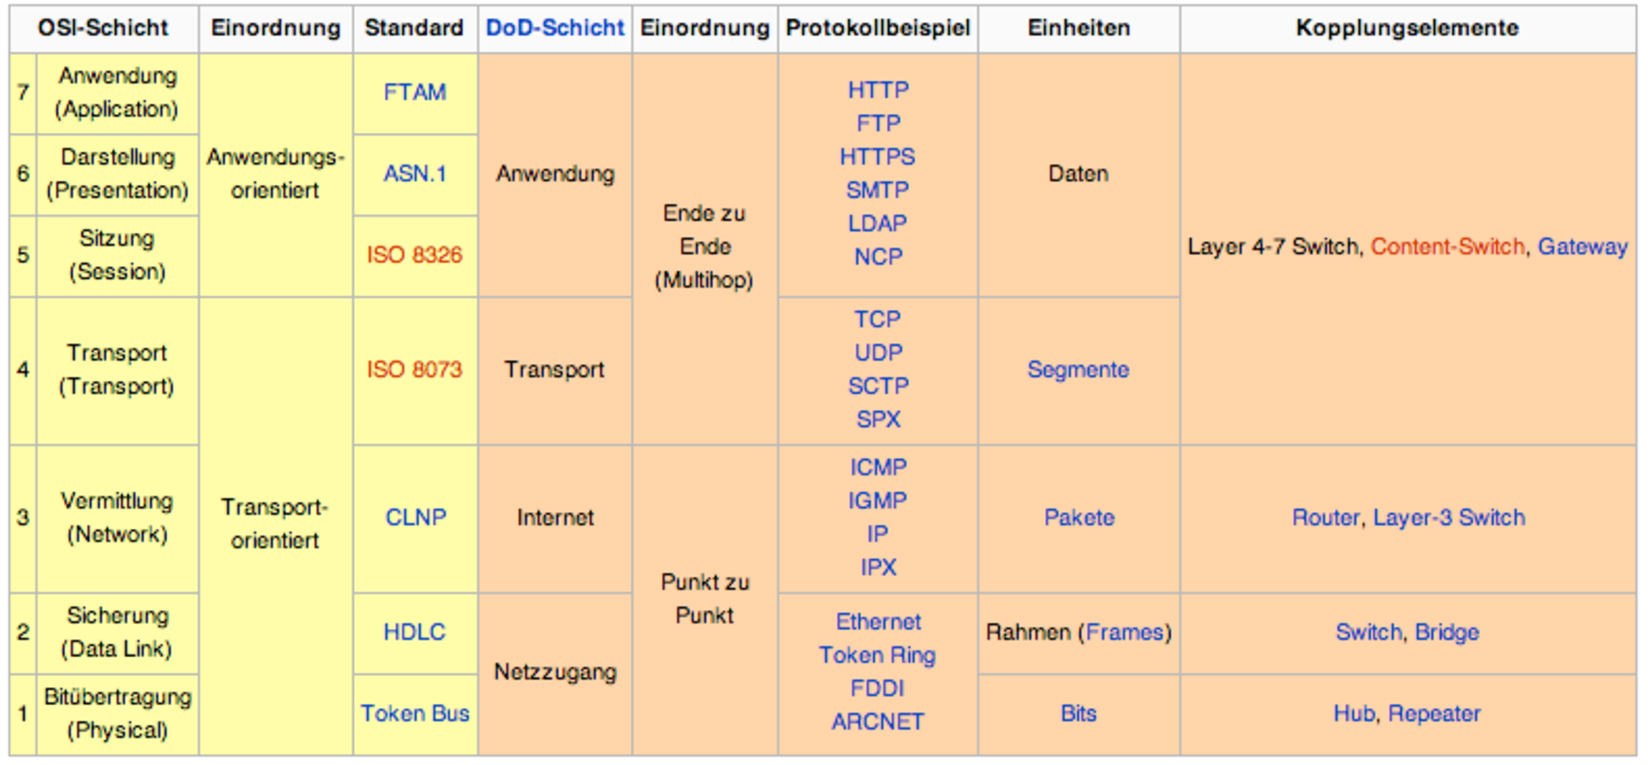
\includegraphics[scale=0.6]{figures/osi.pdf}
\caption{OSI Referenzmodell}
\label{osi}
\end{center}
\end{figure}

\subsection{OSI-Referenzmodell}

\begin{table}[H]
\begin{center}
\begin{tabular}{llll}
 & DE & EN & Beschreibung \\
\toprule
7 & Anwendung & Application & \\
\midrule
6 & Darstellung & Presentation & \\
\midrule
5 & Sitzung & Session & \\
\midrule
4 & Transport & Transport & \\
\midrule
3 & Vermittlung & Network & \\
\midrule
2 & Sicherung & Data Link & \\
\midrule
1& Bit\"ubertragung & Physical &  \\
\bottomrule
\end{tabular}
\caption{OSI-Referenzmodell}

\end{center}
\label{default}
\end{table}%


\subsection{Internet-Referenzmodell}

\begin{table}[H]
\begin{center}
\begin{tabular}{ll}
 Name  & OSI-Schicht \\
\toprule
 Anwendung &  5,6,7\\
  \\
   \\
\midrule
Transport &  4\\
\midrule
Internet & 3 \\
\midrule
Netzzugang & 1,2 \\
 \\
\bottomrule
\end{tabular}
\caption{OSI-Referenzmodell}

\end{center}
\label{default}
\end{table}%

\subsection{Dateneinheiten im Schichtenmodell}


\paragraph{(N)-\underline{I}nterface \underline{D}ata \underline{U}nit.} Die (N)-IDU ist die Dateneinheit, die die (N+1)-Schicht an die (N)-Schicht \"uber den Dienstzugangspunkt \"ubergibt. Sie besteht aus der (N)-SDU und der (N)-ICI.

\paragraph{(N)-\underline{S}ervice \underline{D}ata \underline{U}nit.} Die (N)-SDU entspricht den Daten der (N+1)-Schicht, die transparent weitergegeben werden. Sie entspricht der (N+1)-PDU.

\paragraph{(N)-\underline{I}nterface \underline{C}ontrol \underline{I}nformation.} Die (N)-ICI enth\"alt Information \"uber den auszuf\"uhrenden Dienst, z.B. Parameter des Dienstes oder L\"ange der (N)-SDU. Sie wird in der (N)-Schicht abgetrennt und verworfen.

\paragraph{(N)-\underline{P}rotocol \underline{C}ontrol \underline{I}nformation.} Die (N)-PCI enth\"alt Information, die zwischen (N)-Protokollinstanzen ausgetauscht wird, um den Protokollablauf zu steuern. 

\paragraph{(N)-\underline{P}rotocol \underline{D}ata \underline{U}nit.} In der (N)-Schicht werden (N)-SDU und (N)-PCI zur (N)-PDU zusammengef\"ugt.


\begin{figure}[H]
\begin{center}
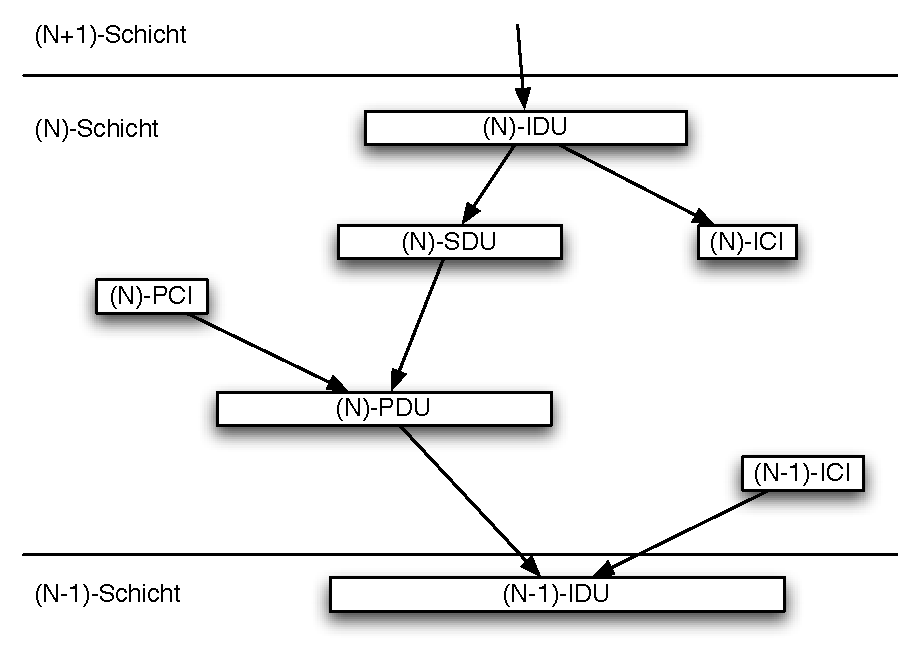
\includegraphics[scale=0.6]{figures/Schichten.pdf}
\caption{Dateneinheiten im Schichtenmodell}
\label{default}
\end{center}
\end{figure}


\section{Bit\"ubertragungsschicht (Physical Layer)}



\subsection{Modulation}


\paragraph{Manchestercodierung. } Eine Signalpegel\"anderung in der Intervallmitte codiert
 $$1 \qquad High \rightarrow Low$$
 $$0\qquad Low \rightarrow High$$


\paragraph{Amplitudenmodulation.} Bits werden durch unterschiedliche Amplitude einer Schwingung moduliert.

\paragraph{Frequenzmodulation.} Bits werden durch unterschiedliche Frequenzen einer Schwingung moduliert.

\paragraph{Phasenmodulation. } Bits werden durch eine Phasendrehung der Schwingung um 180 Grad unterschieden.


\subsection{Betriebsarten}

\begin{description}
\item[Simplex] Kommunikation nur in eine Richtung, z.B. Telex, Feuermelder
\item[Duplex] Kommunikation gleichzeitig in beide Richtungen, z.B. Telefon
\item[Halbduplex] Kommunikationsrichtung abwechselnd, z.B. Walkie-Talkie
\end{description}


\subsection{Kanalkapazit\"at}


\paragraph{Bandbreite. }

$$B = f_{max} - f_{min} \quad [Hz]$$


\paragraph{Schrittgeschwindigkeit (Baudrate). } Rate der Signalparameter-Zustandswechsel. 

$$\quad  \qquad [baud = \frac{1}{s}]$$

Bei isochronen Digitalsignalen ist $s_{max}  = \frac{1}{T}$ mit Schrittdauer $T$.

$$s_{max} = 2 \cdot B$$


\paragraph{Signal-Rausch-Abstand (Signal-Noise-Ratio)} ist das Verh\"altnis von Signalst\"arke zur St\"arke des Rauschens.

$$ SNR =  10 \ log_{10} \ \frac{P_{signal}}{P_{noise}} \qquad [dB]$$

Bei gegebener Kapazit\"at und Bandbreite ist 
$$SNR = 10 \ log_{10} \ ( 2^ \frac{C}{B} - 1)$$


\paragraph{\"Ubertragungsgeschwindigkeit (Bitrate, Datenrate). }

$$ \qquad [\frac{bit}{s}]$$

\"Ubertragungsgeschwindigkeit entspricht Schrittgeschwindigkeit wenn jeder Schritt ein Bit darstellt.


\paragraph{Kanalkapazit\"at } ist die maximale Datenrate.
Ein idealer Kanal ohne Rauschen kann eine beliebige Datenrate durch die Anzahl der Signalstufen $M$ realisieren.
$$C = s_{max} \cdot ld(M)$$

Mit Rauschen ist die maximale Datenrate nach \textsc{Nyquist}

$$C = B \cdot ld(1 + \frac{P_{signal}}{P_{noise}})  $$


\paragraph{Signalstufen}

$$C = s_{max} \ ld(M) \quad \Rightarrow \quad M = 2^{\frac{C}{s_{max}}}$$


\subsection{Leitungskapazit\"at, Laufzeiten}

\paragraph{Sendezeit} ist die Zeit, die ben\"otigt wird, um die Daten auf das Medium zu legen. Es gilt 
$$T_{s} = \frac{L}{d}$$
mit Datenvolumen $L$ und Daten\"ubertragungsrate $d$.


\paragraph{Ausbreitungszeit} ist die Laufzeit der Signale 
\"uber das Medium von Sender zu Empf\"anger. Es 
gilt 
$$ T_{a} = \frac{l}{v}$$

\paragraph{\"Ubertragungsdauer}
$$T_{ges} = T_{s} + T_{a}$$

\paragraph{Ausbreitungsgeschwindigkeit} In \"ublichen Medien (Kabel, Glasfaser) ist

$$ v \approx \frac{2}{3} \ c \approx 200 \ 000 \frac{km}{s}$$

\paragraph{Bandbreiten-Verz\"ogerungs-Produkt} ist das Datenvolumen, das sich w\"ahrend der \"Ubertragung auf dem Medium befindet.

$$L = d \cdot T_{a}$$

\paragraph{Auslastung des Mediums } ist das Verh\"altnis von tats\"achlicher zu m\"oglicher Datenrate.

$$U = \frac{d}{d_{max}}$$


\section{Sicherungsschicht (Data Link Layer)}

\paragraph{Aufgaben der Sicherungsschicht.}
\begin{itemize}
\item Fehlererkennung, z.B. durch CRC
\item Fehlerbehebung, z.B. durch Quittungen und Sendewiederholungen
\item Strukturierung des Datenstroms, z.B. durch Sequenznummern
\item Medienzugangskontrolle, z.B. durch CSMA/CD
\end{itemize}

\paragraph{Unterteilung.} Die Sicherungsschicht kann in zwei Unterbereiche eingeteilt werden:
\begin{description}
\item[\underline{L}ogical \underline{L}ink \underline{C}ontrol] Sicherung der Punkt-zu-Punkt-Verbindung gegen Verf\"alschung, Verlust und Reihenfolgenvertauschung; Flusskontrolle, Strukturierung der \"Ubertragung
\item[\underline{M}edium \underline{A}ccess \underline{C}ontrol] Zugangskontrolle f\"ur ein geteiltes Medium
\end{description}




\subsection{Fehlererkennung}

\paragraph{Paketfehlertypen.} Ein zuverl\"assiger Dienst vermeidet folgende Fehlertypen:
\begin{itemize}
\item Verlust
\item Duplizierung
\item Vertauschung der Reihenfolge
\item Phantom-Dateneinheiten
\end{itemize}



\paragraph{Parit\"atsbit. } Mit einem Parit\"atsbit kann man eine ungerade Anzahl von Fehlern erkennen.

\paragraph{\underline{F}rame \underline{C}heck \underline{S}equence} bezeichnet eine Pr\"ufsumme, die zu einem Datenblock (Frame) hinzugef\"ugt 
wird, um Fehlererkennung oder Fehlerkorrektur zu erm\"oglichen.

\paragraph{\underline{C}yclic \underline{R}edundancy \underline{C}heck}
Hierbei wird die Datensequenz als Polynom betrachtet und ein 
Generatorpolynom festgelegt, das Sender und Empf\"anger bekannt ist. Die Datensequenz wird vor dem Senden durch das Generatorpolynom divivdiert. Der Rest der Division wird an die Datensequenz (als \emph{FCS}) angeh\"angt und beides wird \"ubermittelt. Der Empf\"agner f\"uhrt wiederum die Polynomdivision durch $G$ durch. Falls hierbei kein Rest bleibt, wurde die Sequenz entweder fehlerfrei \"ubertragen, oder die Sequenz ist fehlerhaft, hat aber weiterhin $G$ als Faktor, was sehr unwahrscheinlich ist.

Gegeben sei die Datensequenz $M$ und das Generatorpolynom $G$. 
\begin{enumerate}
\item Multipliziere $M$ mit $2^d$, wobei $d$ der Grad von $G$ ist. Das entspricht dem Anh\"angen von $d$ Nullen an $M$.
$$M' = M \cdot 2^d$$
\item Dividiere $M'$ modulo durch $G$. 
$$C = M' \ mod \ G$$
\item F\"uge $C$ an die Datensequenz an.
$$\tilde{M} = M' + C$$
\item \"Ubertrage $\tilde{M}$
\item Dividiere die empfangene Sequenz modulo durch das Generatorpolynom.
$$C' = \tilde{M} \ mod \ G$$
Wenn $C' = 0$, dann war die \"Ubertragung mit hoher Wahrscheinlichkeit fehlerfrei.
\end{enumerate}

\paragraph{CRC: Implementierung als Schieberegister}

\subsection{Flusskontrolle}

\paragraph{Ziel.} Flusskontrolle dient der Anpassung der \"Ubertragungsrate an die Verarbeitungskapazit\"aten des Empf\"angers.

\paragraph{Anzahl der Sequenznummern mit Sliding Window.} Gegeben seien die Datenrate des Mediums $d$ , die Gr\"o{\ss}e einer Dateneinheit $S$, sowie die Lebenszeit einer Dateneinheit $T_{l}$. Eine Sendewiederholung findet maximal nach $T_{w}$ statt und der Empf\"anger quittiert den Erhalt der Dateneinheit nach maximal $T_{q}$. Dann ist eine untere Schranke f\"ur die ben\"otigte Bitanzahl $n$ gegeben durch 
$$2^n \ Dateneinheiten \ge (2 T_{l} + T_{w} + T_{q}) \cdot D $$
wobei $D = \frac{d}{S}$ die Dateneinheiten-Rate auf dem Medium ist.

\paragraph{Implizite Flusskontrolle } bezeichnet die Drosselung der Datenrate durch das Zur\"uckhalten der Quittungen. Dieses Verfahren ist problematisch:
Wartet der Sender zu lange auf eine Quittung, so wird nach dem Timeout die Dateneinheit erneut gesendet, was die Resourcen von Sender und Empf\"anger sowie die Kapazit\"at des Mediums beansprucht.

\paragraph{\underline{A}utomatic \underline{R}epeat Re\underline{q}uest} steht f\"ur die automatische Wiederholung verlorengegangener oder besch\"adigter Dateneinheiten.

\subsubsection{Stop-and-Wait}
\paragraph{Stop-and-Wait} ist ein einfaches ARQ-Verfahren. Dabei wartet der Sender auf die Quittung zu einer gesendeten Dateneinheit, bevor er die n\"achste verschickt. Falls vor dem Timeout keine Quittung eintrifft, wird die Dateneinheit wiederholt.


\paragraph{\"Ubertragunszeit bei Stop-and-Wait.} Unter der Annahme, dass Verarbeitungsdauer und Gr\"o{\ss}e der Quittung vernachl\"assigbar sind, erreicht die Quittung den Sender nach $T_{s} + 2 \cdot T_{a}$. Damit ist die gesamte \"Ubertragungszeit f\"ur $n$ Dateneinheiten

$$T_{ges} = (T_{s} + 2 \cdot T_{a}) \cdot n$$


\paragraph{Auslastung bei Stop-and-Wait.} Die Auslastung des Mediums beim Stop-and-Wait-Verfahren ist das Verh\"altnis von Sendezeit zur Summe aus Sende- und Wartezeit:

$$U = \frac{T_{s}}{T_{s} + 2 T_{a}}$$


\paragraph{Leistungsf\"ahigkeit im Fehlerfall.} Gegeben sei die Fehlerwahrscheinlichkeit $p$.

$$U = \frac{1-p}{2a + 1}$$

\subsubsection{Go-Back-N}

\paragraph{Prinzip.} Der Sender kann einge gewisse Anzahl von Dateneinheiten (Fenstergr\"o{\ss}e $W$) senden, bevor er eine Quittung empfangen muss. Nach dem Senden der Dateneinheiten $D_{i}, \dots, D_{i+W-1}$ wartet er auf das Eintreffen einer Quittung. Sobald die Quittung $ACK_{i}$ eintrifft, schickt er $D_{i+W}$. Hat der Sender nach Ablauf des Timers keine Quittung f\"ur $D_{i}$ erhalten, wiederholt er alle Dateneinheiten $D_{i}, \dots, D_{i+W-1}$.

 Beim Erhalt einer erwarteten Dateneinheit $D_{i}$ schickt der Empf\"agner die Quittung $ACK_{i}$. Erh\"alt er eine Dateneinheit $D_{j}$ mit $j > i+1$, so wird sie verworfen und die Quittung $ACK_{i}$ wiederholt, solange bis $D_{i+1}$ eintrifft, die dann mit $ACK_{i+1}$ quittiert wird.


\paragraph{Auslastung in Abh\"angigkeit von der Fenstergr\"o{\ss}e.} Das Fenster kann so gro{\ss} sein, dass der Sender kontinuierlich senden kann, oder er muss nach Ausnutzung des Fensters auf die Quittung warten. Im ersten Fall wird die Kapazit\"at des Mediums voll ausgenutzt.

$$ U (W, a) =\left\{ \begin{array}{cl} 
	1 & \mbox{wenn } W \ge 2 a + 1 \\
	 \frac{W}{2a + 1} & \mbox{wenn } W < 2 a + 1
\end{array}\right. $$

$$a = \frac{T_{a}}{T_{s}}$$

\subsection{Medienzugangskontrolle}

\subsubsection{Medienzugangsverfahren}

\paragraph{Raummultiplex} Einteilung des Raumes in Sektoren durch gerichtete Antennen, dedizierte Leitungen etc; Beispiel: Zellenstruktur in Mobilfunknetzen
\paragraph{Zeitmultiplex} Kanal belegt gesamten Frequenzraum f\"ur eine gewisse Zeit; Beispiel: Ethernet
\paragraph{Frequenzmultiplex} Einteilung der verf\"ugbaren Bandbreite in Frequenzabschnitte; Beispiel: UKW-Radio
\paragraph{Codemultiplex} Kan\"ale operieren gleichzeitig auf derselben Frequenz; durch Verkn\"upfung des Signals mit einem eindeutigen Code k\"onnen die Kan\"ale vom Empf\"anger wieder getrennt werden

\subsubsection{CSMA/CD (Carrier Sense Multiple Access with Collision Detection)}

CSMA/CD ist ein Zeitmultiplex-Verfahren bei konkurrierendem Zugriff auf das Medium.

\paragraph{Ablauf.} 
\begin{enumerate}
\item \emph{Listen before Talk}: Endsystem pr\"uft, ob das Medium frei ist
\item Falls Medium frei beginnt das Endsystem zu senden
\item \emph{Listen while Talk}: Zur Erkennung von Kollisionen h\"ort der Sender w\"ahrend des Sendens das Medium ab
\item im Kollisionsfall: Sendeunterbrechung, Jamming-Signal
\item Wiederholung der Sendung, geregelt durch Backoff-Algorithmus
\end{enumerate}

\paragraph{Mindestl\"ange der Dateneinheit.} Eine Voraussetzung f\"ur CSMA/CD ist, dass das Senden der Dateneinheit nach der zweifachen Signallaufzeit noch nicht beendet sein darf. Daraus ergibt sich eine Mindestl\"ange f\"ur die Dateneinheit, die durch das Padding-Feld der Dateneinheiten sichergestellt wird.

\paragraph{CSMA/CD-Dateneinheit}
\begin{table}[H]
\begin{center}
\begin{tabular}{lll}
Abk\"urzung & L\"ange [bit] & Beschreibung \\
\toprule
PR & 56 & Pr\"aambel zur Synchronisation \\
SD & 8 & Start-of-Frame Delimiter zeigt Beginn an \\
DA & 16/48 & Destination Address, MAC-Adresse des Ziels \\
SA & 16/48 & Source Address, MAC-Adresse der Quelle \\
Length & 16 & Anzahl der Oktette im Datenfeld \\
Data & $\le$ 12000 & Datenfeld, max. 1500 Oktette \\
PAD & optional & Padding um auf n\"otige Mindestl\"ange zu erg\"anzen \\
FCS & 32 & Frame Check Sequence, CRC-32 \\
\bottomrule
\end{tabular}
\caption{Felder einer CSMA/CD-Dateneinheit}

\end{center}
\label{default}
\end{table}%




\subsection{Lokale Netze}

\subsection{Ethernet}

\paragraph{Topologie.} Beim Ethernet sind die Endsysteme in Sterntopologie verbunden.

\subsection{Token Ring}

\paragraph{Topologie.} Beim Token Ring sind die Endsysteme jeweils Punkt-zu-Punkt zu einem Ring verbunden. 

\paragraph{Ablauf.}Token Ring erm\"oglicht kontrollierten Zugriff auf das Medium mittels eines zirkulierenden Senderechts (Token). Empf\"angt ein Endsystem das Token, so hat es f\"ur eine bestimmte Zeit das Recht zu senden (Token Holding Time). Die gesendeten Daten kommen nach dem Umlauf im Ring wieder beim Sender an, der diese wieder vom Ring nimmt. Danach gibt er das Token an das nachfolgende System weiter.

\paragraph{Echtzeit.} Token Ring ist f\"ur Echtzeitanwendungen geeignet, da eine maximale Wartezeit  zwischen Sendewunsch und Anfang des Sendens garantiert werden kann:
$$Wartezeit_{max} = (n-1) \cdot Sendezeit(Datenmenge_{max}) + Tokenumlaufzeit$$

\paragraph{Quittierung.} Ein Endsystem im Token Ring kann die Dateneinheit \"andern, bevor es diese weitergibt. Der Empf\"anger kann also den Erhalt einer Dateneinheit quittieren, indem er z.B. ein bestimmtes Bit setzt. Der Sender erkennt diese Quittung w\"ahrend er die Dateneinheit vom Ring nimmt.

\paragraph{Aktiver Anschluss ans Medium.} Beim Token Ring sind die Endsysteme aktiv ans Medium angeschlossen. Jedes System regeneriert die erhaltene Dateneinheit und schickt sie weiter, agiert somit als Verst\"arker. Das erm\"oglicht gr\"o{\ss}ere Leitungsl\"ange. Die Regenerierung ist allerdings mit Verz\"ogerung verbunden. F\"ur den Anschluss neuer Systeme an das Medium muss das Medium unterbrochen werden.





\subsection{\underline{H}igh-Level \underline{D}ata \underline{L}ink \underline{C}ontrol}


\paragraph{Phasen.}

\begin{enumerate}
\item Verbindungsaufbau
\item Datentransfer
\item Verbindungsabbau
\end{enumerate}

\paragraph{Flag. } Die eindeutige Bitsequenz
$$ \mathtt{01111110}$$
 wird verwendet, um Anfang und Ende einer Dateneinheit zu signalisieren. Ein Autreten des Flags in den Nutzdaten wird durch \emph{Bitstopfen} verhindert. Hierbei wird nach 5 aufeinanderfolgenden Einsen eine Null eingef\"ugt, die vom Sender wieder entfernt wird.


\paragraph{Codetransparenz } bedeutet, dass es f\"ur eine Anwendung transparent bleibt, welche Mechanismen und Codes zur \"Ubertragung verwendet werden. So wird z.B. durch Bitstopfen auf der Sicherungsschicht erreicht, dass die Anwendung die Existenz einer ausgezeichneten Bitfolge als  Anfangs- und Endflag bei der Codierung ihrer Daten nicht ber\"ucksichtigen muss.

\paragraph{Piggyback Acknowledgement} verwendet f\"ur das Senden einer Best\"atigung keine separate Dateneinheit, sondern benutzt eine Dateneinheit mit, die selber Nutzdaten enth\"alt.



\section{Vermittlungsschicht (Network Layer)}


\subsection{Vermittlungsarten}

\begin{description}
\item[Leitungsvermittlung] durchgehender, nichtspeichernder \"Ubertragungskanal zwischen den Endsystemen; Bitfolgen reihenfolgetreu; Vermittlung in den Zwischensystemen erfordert keine zus\"atzliche Kontrollinformation zur Adressierung; starre Leitungszuordnung; nur verbindungsorientierter Dienst; Beispiel: ISDN
\item[Speichervermittlung]  Zwischensysteme verf\"ugen \"uber Speicher; flexible Ressourcenzuordnung und Fehlerbehandlung; verbindungsloser Dienst m\"oglich; komplex; Verz\"ogerung, Reihenfolgevertauschung m\"oglich;
 \begin{description}
\item[Nachrichtenvermittlung]
\item[Paketvermittlung] Vermittlung aufgrund von Vermittlungsinformation in den Dateneinheiten
\begin{description}
\item[Datagramme]
\item[virtuelle Verbindung]
\end{description}

\end{description}

\end{description}

\subsection{\underline{I}ntegrated \underline{S}ervices \underline{D}igital \underline{N}etwork}

\paragraph{Kan\"ale.}
\begin{itemize}
\item 1 D-Kanal zur Signalisierung, 16 kbit/s
\item 2 B-Kan\"ale zur Sprach-/Daten\"ubertragung, 64 kbit/s
\end{itemize}


\subsection{\underline{I}nternet \underline{P}rotocol}

\paragraph{Dienst.} IP stellt einen unzuverl\"assigen und verbindungslosen Dienst zur Verf\"ugung.

\paragraph{\underline{T}ime \underline{T}o \underline{L}ive} ist ein Feld im Header einer IP-Dateneinheit. Dieser Wert wird vom Sender gesetzt und gibt die maximale Anzahl an Hops an, die das Paket durchlaufen darf. In jedem Router, den das Paket durchl\"auft, wird der Wert um 1 dekrementiert. Pakete mit einem TTL-Wert von 0 werden gel\"oscht und es wird eine ICMP-Nachricht an den Absender geschickt. Durch TTL wird die Wegewahl unterst\"utzt und es werden umherirrende Pakete vermieden.

\subsection{Segmentierung und Reassemblierung}

\paragraph{Motivation.} Existieren auf einem Pfad durch das Netzwerk unterschiedliche \underline{M}aximum \underline{T}ransfer \underline{U}nits, so m\"ussen eventuell Dateneinheiten beim \"Ubergang segmentiert und sp\"ater reassembliert werden. Die Reassemblierung sollte nicht schon in zwischenliegenden Routern erfolgen, da sich Routen w\"ahrend der \"Ubertragungszeit einer fragmentierten Einheit \"andern k\"onnen oder einzelne Fragmente verlorengehen k\"onnen.

\subsection{Zustands\"ubergangsdiagramm}

$Stimulus ; Reaktion$

\paragraph{Dienstprimitive beim Initiator.}

\begin{description}
\item[TConReq] Anforderung eines Verbindungsaufbaus
\item[TConConf] Verbindungsaufbau erfolgreich
\item[TDisInd] Beantworter lehnt Verbindungsaufbau ab
\item[TPAboInd1] Abbruch durch \"Ubertragungsabschnitt
\end{description}

\paragraph{Dienstprimitive beim Beantworter.}

\begin{description}
\item[TConRsp] Best\"atigung des Verbindungsaufbauwunschs
\item[TDisReq] Ablehnung des Verbindungsaufbauwunschs
\item[TConInd] Mitteilung des Verbindungsaufbauwunschs
\item[TPAboInd2] Abbruch durch \"Ubertragungsabschnitt
\end{description}

\paragraph{Protokollinstanz. }

\paragraph{Dienstspezifikation.} Die Dienstspezifikation beschreibt das an der Dienstschnittstelle von au{\ss}en betrachtete Verhalten des Dienstes.

\paragraph{Protokollspezifikation.} Die Protokollspezifikation legt durch Regeln und Formate das Kommunikationsverhalten zweier Protokollinstanzen fest.






\subsection{Routing}

\paragraph{statisches Routing vs adaptives/dynamisches Routing.} Bei statischen Routing-Algorithmen ist die Routing-Tabelle f\"ur l\"angere Zeit fixiert. Adaptives oder dynamisches Routing basiert dagegen darauf, dass die Routing-Tabellen laufend angepasst werden.

\subsubsection{Distanz-Vektor-Routing}

\paragraph{Prinzip.}Beim Distanz-Vektor-Routing kennt kein Knoten die komplette Route von der Quelle zur Senke. Der Knoten kennt nur die Distanz zu allen anderen Knoten.

\paragraph{Distanz-Vektor-Tabelle.} Die Distanz-Vektor-Tabelle enth\"alt eine Zeile f\"ur jedes m\"ogliche Ziel und eine Spalte f\"ur jeden direkten Nachbarn (Next Hop). Knoten $X$ m\"ochte eine Nachricht \"uber den direkten Nachbarn $Z$ an $Y$ verschicken.

$$X \to Z \to Y$$

Dann ist der Eintrag in der Distanz-Vektor-Tabelle von $X$ gegeben durch die Summe aus Kantengewicht zwischen $X$ und $Z$ und dem minimalen Eintrag in der $Y$-Zeile der Tabelle von $Z$:

$$D^X (Y,Z) = c(X,Z) + \min_{v}\{ D^Z (Y,v)\}$$

\paragraph{Algorithmus.} Zun\"achst kennt jeder Knoten nur die Distanzen zu seinen direkten Nachbarn, d.h. die Eintr\"age auf der Diagonalen der Tabelle. Diese schickt er an alle direkten Nachbarn, die ihre eigenen Distanzen entsprechend aktualisieren. Solange ein Knoten nach einer Aktualisierung neue k\"urzeste Wege kennt, schickt er sie an seine Nachbarn.

\begin{algorithm}[htbp]
\caption{Distanz-Vektor-Algorithmus f\"ur Knoten $s$}

\end{algorithm}


\subsubsection{Link State Routing} 

\paragraph{Prinzip.} Die Routing-Tabelle jedes Routers enth\"alt die k\"urzesten Wege zu allen anderen Routern. Zur Berechnung der k\"urzesten Wege kann z.B. Dijkstras Algorithmus eingesetzt werden. Dadurch, dass jeder Knoten Informationen \"uber seine adjazenten Kanten broadcastet, kann der einzelne Knoten einen Graphen des gesamten Netzes konstruieren und die k\"urzesten Wege berechnen.

\paragraph{}

\begin{algorithm}[H]
\caption{Dijkstras Algorithmus}
\KwIn{Graph $G = (V,E)$,Startknoten $s$, symmetrische, positive Kantengewichtsfunktion $c: E \to \mathbb{R}^+$}
$N \gets \{ s \}$ \\
\For{$u \in V \backslash \{ s \}$} {
	\eIf{$\{s,u\} \in E$}{
		$d(u) \gets c(s,u)$ \\
		$p(u) \gets s$ \\
	}{
		$d(u) \gets \infty$ \\
	}
\While{$N \neq V$} {
	$N \cup \{ u \} ,  u \not \in N \wedge d(u) = \min (d)$\\
	\For{ $\{ u, v\} \in E$} {
		\If{$d(v) + c(u,v) < d(v)$} {
			$d(v) \gets d(v) + c(u,v)$ \\
			$p(v) \gets u$ \\
		}
	}
}
}

\end{algorithm}


\paragraph{Kostenfunktion.} Die Kostenfunktion der Kanten kann von verschiedenen Faktoren abh\"angig gemacht werden, z.B.
\begin{itemize}
\item physikalisches Medium
\item Verkehrsaufkommen
\item politische Bestrebungen der Netzbetreiber
\item Dienstg\"utemerkmale, z.B. garantierte Bandbreiten, Latenzzeiten oder Zuverl\"assigkeitsgarantien
\end{itemize}




\subsection{IP-Adressierung}

\paragraph{Subnetzmaske} Die Subnetzmaske zerlegt eine IP-Adresse in Netzwerk-Teil und Endsystem-Teil. Sie ist eine Bitsequenz der Form $1^m0^n$. Den Netzwerkteil einer IP-Adresse erh\"alt man durch und-Verkn\"upfung von IP-Adresse und Subnetzmaske in Bin\"ardarstellung.

$$IPAdresse \wedge Subnetzmaske = Netzwerkteil$$

\paragraph{Adressbereich.}Zur Darstellung eines Adressbereiches wird die Anzahl der 1er-Bits in der Subnetzmaske an die IP-Adresse angef\"ugt. Eine IP-Adresse $a$ liegt im Adressbereich $b/m$, wenn die ersten $m$ Bits von $a$ und $b$ \"ubereinstimmen.


\subsection{\underline{A}ddress \underline{R}esolution \underline{P}rotocol} 

\paragraph{Aufgabe.}Das Address Resolution Protocol ist f\"ur die Zuordnung

$$\mathtt{IP-Adresse} \leftrightarrow \mathtt{MAC-Adresse}$$

zust\"andig.

\paragraph{Ablauf.}
\begin{enumerate}
\item suche im eigenen ARP-Cache; wenn Eintrag nicht gefunden:
\item sende ARP-Request mit gesuchter IP-Adresse, eigener IP-Adresse und eigener MAC-Adresse an alle (Broadcast)
\item Besitzer der gesuchten IP-Adresse sendet ARP-Reply mit seiner MAC-Adresse zur\"uck
\item lege Wert im ARP-Cache ab
\end{enumerate}


\subsection{\underline{D}omain \underline{N}ame \underline{S}ystem}

\paragraph{DNS-Anfrage.} Eine DNS-Anfrage zur Aufl\"osung eines Domainnamen nach einer IP-Adresse stellt entweder

a) rekursive Anfragen: 
\begin{itemize} 
\item Der Client sucht im lokalen Cache.
\item Der Client befragt den Cache des lokalen DNS-Servers.
\item Der DNS-Server befragt den Cache (bzw. Datenbank im Falle autoritativer Server) anderer fest definierter DNS-Server.
\item Der DNS-Server f\"uhrt eine sukzessive Aufl\"osung beginnend bei DNS-Rootservern durch
\end{itemize}
Dabei wird jede erhaltene Antwort im lokalen Cache f\"ur einige Tage gespeichert, um die Anfragen m\"oglichst direkt beantworten zu k\"onnen. \\

b) iterative Anfragen: Der Client befragt der Reihe nach weitere Server, wenn er keine Antwort erh\"alt.

\paragraph{Effizienz.} Aus Effizienzgr\"unden sollte ein Endsystem meist den topologisch nahegelegensten DNS-Server zur Adressaufl\"osung verwenden.

\paragraph{Transport.} Der Transport von DNS-Anfragen wird \"uber UDP abgewickelt. Der mit TCP verbundene Overhead kann vermieden werden, da die Sicherungsmechanismen von TCP nicht ben\"otigt werden.

\paragraph{Hierarchie.} Das DNS ist in einer Baumstruktur organisiert.


\section{Transportschicht (Transport Layer)}


\subsection{\underline{U}ser \underline{D}atagram \underline{P}rotocol}

\subsection{\underline{T}ransmission \underline{C}ontrol \underline{P}rotocol}

\paragraph{Charakteristika.} Eine TCP-Verbindung stellt einen Duplex-Kanal zwischen Sender und Empf\"anger bereit. Sie stellt einen bytestromorientierten Dienst zur Verf\"ugung. TCP nutzt verschiedene Mechanismen um eine zuverl\"assige Verbindung herzustellen:
\begin{itemize}
\item Quittungen zur Entdeckung verlorener Pakete
\item Sequenznummern um Reihenfolge zu gew\"ahrleisten
\item Pr\"ufsumme um Integrit\"at der Daten zu garantieren
\end{itemize}

\paragraph{TCP-Dateneinheit.}

\begin{table}[H]
\begin{center}
\begin{tabular}{lll}
Bezeichnung & L\"ange [bit] & Beschreibung \\
\toprule
 Quellport & 16 & \\
Zielport & 16 & \\
Sequenznummer & 32 & gemessen in Byte\\
Quittung & 32 & n\"achste vom Empf\"anger erwartete Sequenznummer \\
 Offset & & Anzahl der 32-Bit-W\"orter im TCP-Header \\
 reserviert& & \\
 URG & 1 & gesetzt falls Urgent-Pointer verwendet \\
 ACK & 1 & unterscheidet bei SYN=1 TConReq von TConCnf, zeigt Quittung an\\
 PSH & 1 & \"ubergebene Daten sofort weiterleiten \\
 RST & 1 & Zur\"ucksetzen der Verbindung \\
 SYN & 1 & zeigt TConReq oder TConCnf an\\
 FIN & 1 & Sender m\"ochte keine Daten mehr senden\\
  Empfangsfenster & 16 & Fenstergr\"o{\ss}e f\"ur Sender in Byte zur Flusskontrolle \\
  Pr\"ufsumme & 16 & \"uber TCP-Kopf und Daten \\
  Urgent Pointer & 16 & Zeiger auf wichtige Daten\\
  \midrule
  Optionen & $k \cdot 32$ & \\
  \midrule
  Daten & & \\
\bottomrule
\end{tabular}
\caption{Felder einer TCP-Dateneinheit}
\end{center}
\end{table}


\paragraph{Verbindungsaufbau (3-Way Handshake).} Der Verbindungsaufbau wird vom Client initiiert.
\begin{enumerate}
\item TConReq(SYN=1, seq=client-isn) $\rightarrow$
\item $\leftarrow$ TConCnf(SYN=1, ACK=1, seq=server-isn, ack=client-isn + 1)
\item ACK(SYN=0, ACK=1, seq=client-isn + 1, ack=server-isn + 1) $\rightarrow$
\end{enumerate}

\paragraph{Verbindungsabbau.} Bei TCP wird wenn m\"oglicher ein expliziter Verbindungsabbau durchgef\"uhrt, statt die Verbindung per Reset zur\"uckzusetzen, da zum Zeitpunkt des Verbindungsabbaus noch Daten unterwegs sein k\"onnen. Bei einem Reset w\"are es nicht unbedingt erkennbar, welche Daten noch korrekt empfangen wurden. Der Verbindungsabbau kann sowohl vom Client als auch vom Server initiiert werden. Nach dem letzten ACK wird noch gewartet, bevor der lokaler Kontext gel\"oscht wird, da noch Pakete verlorengehen k\"onnten.

\begin{enumerate}
\item FIN $\rightarrow$
\item $\leftarrow$ ACK
\end{enumerate}


\section{Sitzungsschicht (Session Layer)}

\section{Darstellungsschicht (Presentation Layer)}

\section{Anwendungsschicht (Application Layer)}

\subsection{Anwendungsprotokolle}
\begin{description}
\item[\underline{H}yper\underline{T}ext \underline{T}ransfer \underline{P}rotocol] Austausch von HTML-Dokumenten
\item[\underline{F}ile \underline{T}ransfer \underline{P}rotocol] Austausch von Dateien zwischen Dateisystemen
\item[\underline{S}imple \underline{M}ail \underline{T}ransfer \underline{P}rotocol] Transport von elektronischer Post
\end{description}


\begin{figure}[b]
\begin{center}

\includegraphics[scale=0.6]{figures/88x31.png}
\label{default}
\end{center}
\end{figure}

\end{document}
